\documentclass{siproblemset}

\usepackage{multicol}

% SI Session Information
\course{MTH 1321}
\sessionnum{2}
\sessiondate{8/30/21}

\warmup{Concept Review}
\topic{Rates of Change}
\topic{Understanding Limits}
\cooldown{Infinite Limits}

% Worksheet Information
\title{Introduction to Limits}
\sections{Sections 2.1-2.2}
\withnamespace

\begin{document}
    \maketitle
    
    \activity{Warmup}{Concept Review}{Try these problems \textbf{alone} as your peers join the session.}{10 minutes}
    
    \begin{multipartquestion}
        \frq{Derive an expression for the slope of a secant line between the points $(a,f(a))$ and $(a+h,f(a+h))$.}
        \Tinysp
        \frq{What does the slope of a secant line represent?}
        \tinysp
    \end{multipartquestion}

    \frq{What is a tangent line and what does its slope represent?}
    \smallsp
    
    \frq{In your own words, describe what a limit is and/or what it does.}
    \smallsp
    
    \frq{What are the condition(s) for a limit (such as $\lim\limits_{x\to 2}f(x)$) to exist?}
    \Tinysp
   
    \pagebreak
    
    \activity{Activity 1}{Rates of Change}{Work together in your \textbf{breakout rooms} to answer these questions. \textbf{Use a calculator for this section as needed.}}{20 minutes}
    \frq{Estimate the slope of the tangent line to $y=\dfrac{1}{x-3}$ at $x=-2$.}
    \Hugesp
    
    \mcq{A meteor enters Jupiter's atmosphere where its distance traveled (before burning up) is given by the function $s(t)=12.5t^2$ m where $t$ is in seconds.}{
        \task Compute the meteor's average velocity over the time interval $[2,4]$ seconds.
        \hugesp
        \task Estimate numerically the meteor's instantaneous velocity at $t=6$ seconds. Use at least 4 data points for your estimation (two on each side).
    }
    \Hugesp
    
    \mcq{Consider the function $y=4-x$ for the following questions.}{
        \task What is the average rate of change over the interval $x\in[-1,2]$? 
        \Smallsp
        \task What is the instantaneous rate of change at $x=0$?
    }
\pagebreak
    
    \activity{Activity 2}{Evaluating Limits}{Work together in your \textbf{breakout rooms} to answer these questions. \textbf{Use a calculator for this section as needed.}}{20 minutes}
    
    \begin{multipartquestion}
        Find the value of the following limits. If the limit does not exist, find the values of the left-hand and right-hand limits.
        \begin{multicols}{2}
            \frq{$\lim\limits_{x\to -2}f(x)$ and $\lim\limits_{x\to 1}f(x)$}
            \mbox{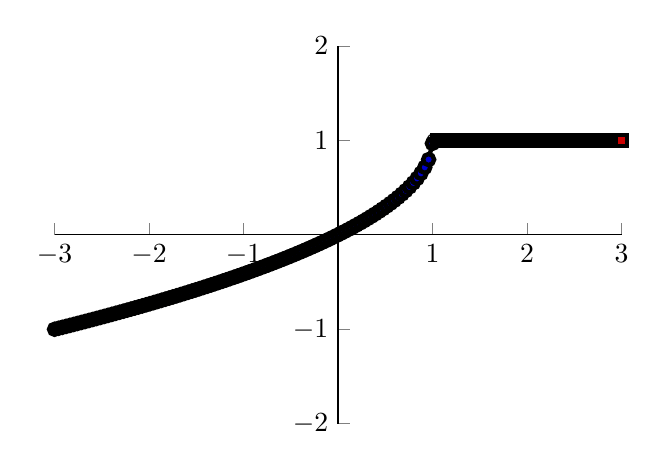
\begin{tikzpicture}[baseline=(current bounding box.north)]
                \begin{axis}[
                x=1.2cm,
                y=1.2cm,
                xmin=-3,
                xmax=3,
                ymin=-2,
                ymax=2,
                axis x line*=middle,
                axis y line*=middle,
                every axis plot/.append style={ultra thick},
                samples=100
                ]
                \addplot+[black, domain=-3:0.999] {1-sqrt(-x+1)};
                \addplot+[black, domain=1.05:3] {1};
                \node at (1,1) {$\circ$};
                \end{axis}
                \end{tikzpicture}}
            \Tinysp
            
            \frq{$\lim\limits_{x\to -2}f(x)$ and $\lim\limits_{x\to 2}f(x)$}
            \mbox{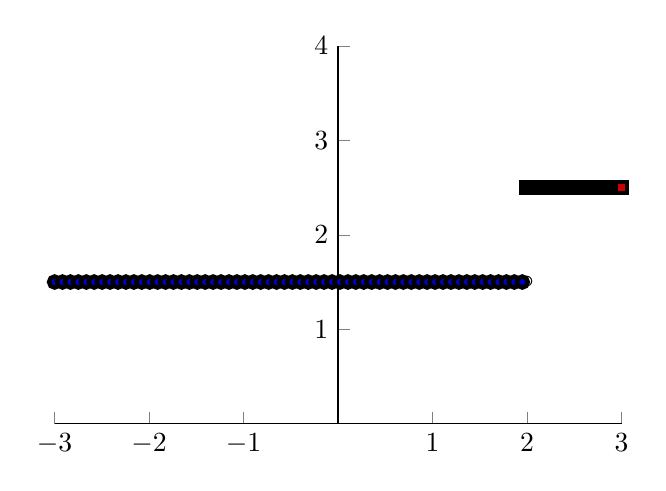
\begin{tikzpicture}[baseline=(current bounding box.north)]
                \begin{axis}[
                    x=1.2cm,
                    y=1.2cm,
                    xmin=-3,
                    xmax=3,
                    ymin=0,
                    ymax=4,
                    axis x line*=middle,
                    axis y line*=middle,
                    every axis plot/.append style={ultra thick},
                    samples=60
                    ]
                    \addplot+[black, domain=-3:1.95] {1.5};
                    \addplot+[black, domain=2:3] {2.5};
                    \node at (2,1.5) {$\circ$};
                    \node at (2,2.5) {\textbullet};
                \end{axis}
            \end{tikzpicture}}
            \Tinysp
        
            
            \columnbreak
        
%            \frq{[(b)]$\lim\limits_{x\to -1}f(x)$ and $\lim\limits_{x\to 0}f(x)$}
%            \mbox{\begin{tikzpicture}[baseline=(current bounding box.north)]
%                \begin{axis}[
%                    x=1.2cm,
%                    y=1.2cm,
%                    xmin=-3,
%                    xmax=3,
%                    ymin=0,
%                    ymax=4,
%                    axis x line*=middle,
%                    axis y line*=middle,
%                    every axis plot/.append style={ultra thick},
%                    samples=100
%                    ]
%                    \addplot+[black, domain=-3:-0.01,restrict y to domain =-20:100] {1/(x+1)^2};
%                    \addplot+[black, domain=0.01:3] {x+1/2};
%                    \node at (0,1) {$\circ$};
%                    \node at (0,0.5) {\textbullet};
%                \end{axis}
%            \end{tikzpicture}}
%            \Tinysp
        
            \frq{$\lim\limits_{x\to 0}f(x)$ and $\lim\limits_{x\to 2.5}f(x)$}
            \mbox{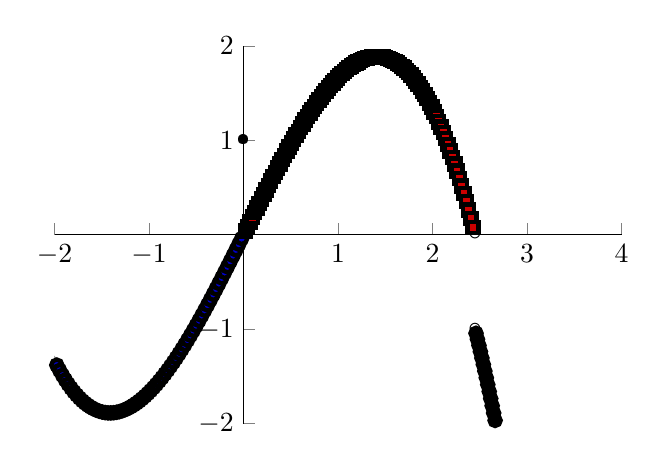
\begin{tikzpicture}[baseline=(current bounding box.north)]
                \begin{axis}[
                    x=1.2cm,
                    y=1.2cm,
                    xmin=-2,
                    xmax=4,
                    ymin=-2,
                    ymax=2,
                    axis x line*=middle,
                    axis y line*=middle,
                    every axis plot/.append style={ultra thick},
                    samples=100
                    ]
                    \addplot+[black, domain=-3:-0.02,restrict y to domain =-20:100] {-x^3/3+2*x};
                    \addplot+[black, domain=0.02:2.43,restrict y to domain =-20:100] {-x^3/3+2*x};
                    \addplot+[black, domain=2.46:4,restrict y to domain =-20:100] {-x^3/3+2*x-1};
                    \node at (0,0) {$\circ$};
                    \node at (0,1) {\textbullet};
                    \node at (2.45,0) {$\circ$};
                    \node at (2.45,-1) {$\circ$};
                \end{axis}
            \end{tikzpicture}}
            \Tinysp
        \end{multicols}
    \Tinysp
    \end{multipartquestion}
    \newpage
    \begin{multipartquestion}
        Use the tables below and optionally a calculator to estimate the value of the following limits numerically. Choose appropriate $x$-values to use. If the limit does not exist, estimate the values of the left-hand and right-hand limits.
        \frq{$\lim\limits_{x\to 0}\dfrac{x^2-4x}{x-4}$\hfill
        \begin{tabular}{ |c|c|c|c|c| } 
            \hline
            \textbf{$x$} & \textbf{$-0.001$} & \textbf{$-0.0001$} & \textbf{$0.0001$} &\textbf{ $0.001$} \\
            \hline
            \textbf{$f(x)$} & \hspace{2cm} & \hspace{2cm} & \hspace{2cm} & \hspace{2cm} \\
            \hline
        \end{tabular}}
        \Smallsp
        \frq{$\lim\limits_{x\to -3}\dfrac{1}{x+3}$\hfill
            \begin{tabular}{ |c|c|c|c|c| } 
                \hline
                \textbf{$x$} & \textbf{$-3.001$} & \textbf{$-3.0001$} & \textbf{$-2.9999$} &\textbf{ $-2.999$} \\
                \hline
                \textbf{$f(x)$} & \hspace{2cm} & \hspace{2cm} & \hspace{2cm} & \hspace{2cm} \\
                \hline
        \end{tabular}}
    \end{multipartquestion}
    \Smallsp
    
    \activity{Cooldown}{Infinite Limits}{Answer these questions as a large group.}{15 minutes}
    \frq{Determine $\lim\limits_{x\to -1.5}f(x)$, $\lim\limits_{x\to 1.5}f(x)$, and $\lim\limits_{x\to 5.5}f(x)$ using the graph of $f(x)$ below. If the limit does not exist, find the values of the left-hand and right-hand limits.}
    \mbox{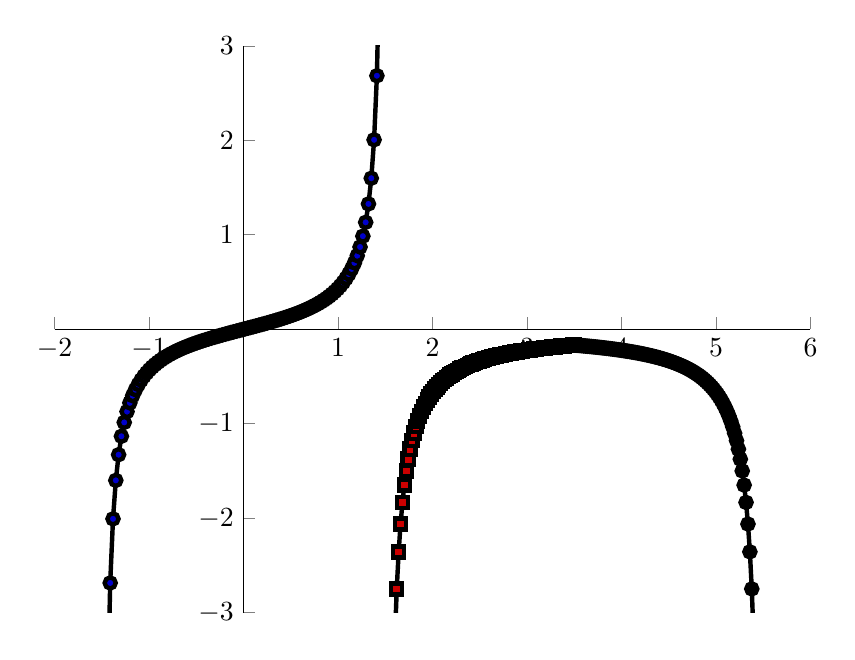
\begin{tikzpicture}[baseline=(current bounding box.north)]
        \begin{axis}[
        x=1.2cm,
        y=1.2cm,
        xmin=-2,
        xmax=6,
        ymin=-3,
        ymax=3,
        axis x line*=middle,
        axis y line*=middle,
        every axis plot/.append style={ultra thick},
        samples=100
        ]
        \addplot+[black, domain=-pi/2+0.1:pi/2-0.1,restrict y to domain =-100:100] {1/4*tan(x/pi*180*pi/3)};
        \addplot+[black, domain=1.5:3.5,restrict y to domain =-20:20] {-(1/3)/(x-1.5)};
        \addplot+[black, domain=3.5:5.5,restrict y to domain =-20:20] {(1/3)/(x-5.5)};
%        \node at (0,0) {$\circ$};
%        \node at (0,1) {\textbullet};
%        \node at (2.45,0) {$\circ$};
%        \node at (2.45,-1) {$\circ$};
        \end{axis}
        \end{tikzpicture}}
    \Tinysp
   
\end{document}